\lstset{
  basicstyle=\ttfamily,
  columns=fullflexible,
  frame=single,
  breaklines=true,
  showlines=true,
  postbreak=\mbox{\textcolor{red}{$\hookrightarrow$}\space},
}

\chapter{Analisis}
\label{chap:analisis}
	Pengumpulan data dalam skripsi ini dilakukan dengan cara studi pustaka.

\section{Analisis Sistem yang Sudah Ada}
\label{sec:analisiskini}
\begin{figure}[H]
	\centering  
	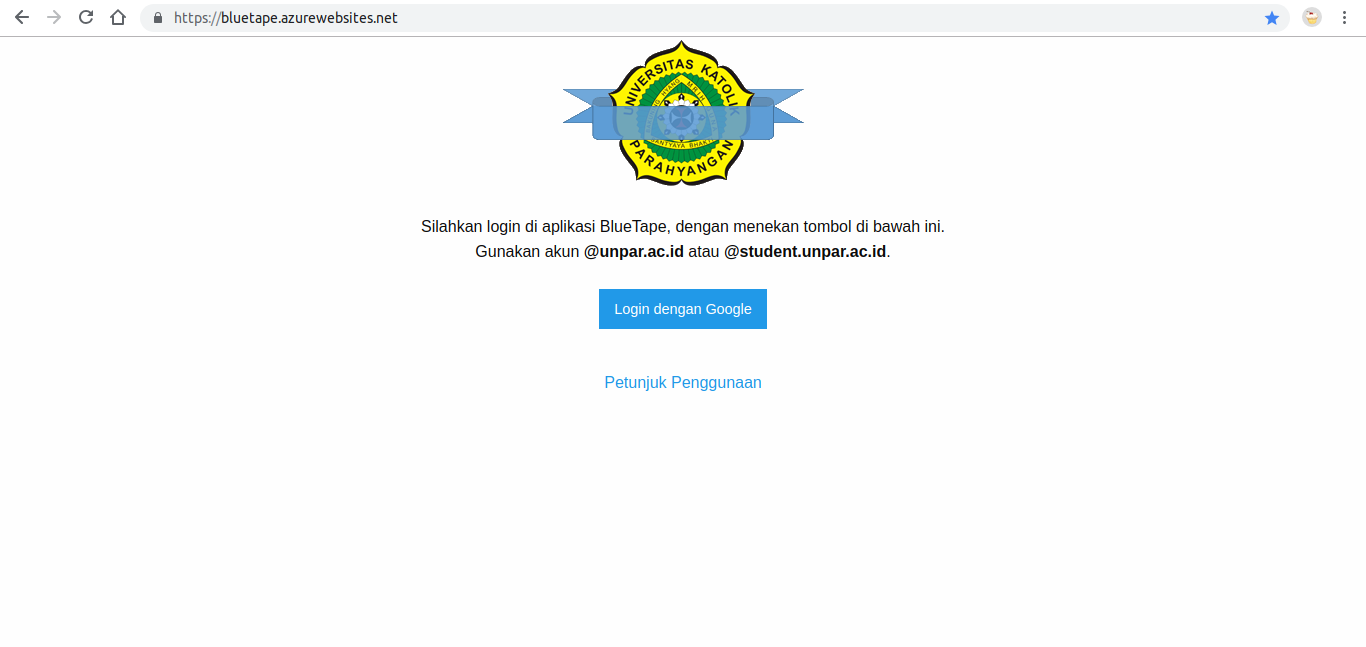
\includegraphics[width=\textwidth]{bluetape-login.png}  
	\caption[Tampilan utama BlueTape]{Tampilan utama BlueTape} 
	\label{fig:bluetape-login} 
\end{figure}

	\textit{BlueTape} adalah perangkat lunak yang berfungsi untuk membantu urusan-urusan \textit{paper-based} di FTIS UNPAR menjadi \textit{paperless}. Pada saat skripsi ini dibuat, BlueTape dapat diakses melalui situs web \url{https://bluetape.azurewebsites.net/} (Gambar~\ref{fig:bluetape-login}). Perangkat lunak ini bersifat \textit{open source}, sehingga kode program BlueTape bisa dipelajari, diubah, dan distribusi oleh siapapun untuk tujuan apapun. Kode program ini dapat diakses di \url{https://github.com/ftisunpar/BlueTape}. BlueTape memanfaatkan CodeIgniter (versi 3.1.4) dan ZURB Foundation.
	
	Pola pengembangan yang dipakai BlueTape adalah MVC (\textit{Model-View-Controller}). MVC (\textit{Model-View-Controller}) adalah sebuah metode untuk membuat perangkat lunak menjadi tiga bagian: \textit{Model, View, dan Controller}. \textit{Model} adalah kelas yang merepresentasikan struktur data. \textit{View} adalah informasi yang disajikan ke pengguna. \textit{Controller} adalah penghubung antara \textit{Model}, \textit{View}, dan sumber daya lain yang dibutuhkan untuk mengolah HTTP \textit{request} dan menghasilkan situs web.

\subsection{Aturan Konstribusi BlueTape}
	Terdapat beberapa aturan apabila ingin berkonstribusi pada pengembangan BlueTape. Aturan-aturan tersebut tertera pada \textit{file} \texttt{CONTRIBUTING.md} (\url{https://github.com/ftisunpar/BlueTape/blob/master/CONTRIBUTING.md}).

	\subsubsection{Pengelompokan Module}
		Perangkat lunak BlueTape dikelompokkan dalam \textit{module}. Setiap \textit{module} memiliki nama yang mengikuti aturan \textit{CamelCase}. Jika beberapa \textit{module} tergabung pada satu topik yang sama, topik tersebut harus digunakan sebagai kata pertama dalam penamaan \textit{module}. Contohnya: apabila nama topik adalah \texttt{Transkrip}, maka contoh nama \textit{module-}nya adalah \texttt{TranskripRequest} dan \texttt{TranskripManage}.
		
		Penamaan dokumen pada \textit{controller}, \textit{view}, \textit{model}, config file, nama tabel, dan migration script menggunakan nama \textit{module} atau topik. Contoh penamaan:
		\begin{itemize}
			\item \textit{Controller}: \texttt{controllers/TranskripRequest.php}, \texttt{controllers/TranskripManage.php}
			\item \textit{View}: \texttt{views/TranskripRequest/*.php}, \texttt{views/TranskripManage/*.php}
			\item \textit{Model} (opsional): \texttt{models/Transkrip/*\_model.php}
			\item \textit{Config} file (opsional): \texttt{config/Transkrip.php}
			\item Nama tabel (opsional): \texttt{Transkrip}
			\item \textit{Migration script} (opsional): \texttt{migrations/20160222120000\_Transkrip\_initial.php}
		\end{itemize} 
	
	\subsubsection{\textit{Model}}
		\textit{Model} dibuat hanya jika fungsi-fungsi di dalamnya digunakan lebih dari sekali. Apabila hanya digunakan sekali, letakkan fungsi pada \textit{controller}.
	
	\subsubsection{Library \texttt{bluetape}}
		Library \texttt{bluetape} berisi fungsi-fungsi yang umum digunakan di BlueTape. Contoh: fungsi untuk konversi \textit{email} ke NPM.
	
	\subsubsection{Hak Akses}
		Hak akses dan nama \textit{module} diatur pada dokumen \texttt{config/modules.php}. Contoh:
\begin{lstlisting}
$config['module-names'] = array(
    'TranskripRequest' => 'Permohonan Cetak Transkrip',
    'TranskripManage' => 'Manajemen Cetak Transkrip'
);

$config['modules'] = array(
    'TranskripRequest' => array('root', 'mahasiswa.ftis'),
    'TranskripManage' => array('root', 'tu.ftis')
);

$config['roles'] = array(
    'root' => 'pascal@unpar\\.ac\\.id',
    'tu.ftis' => '(shao\\.wei)@unpar\\.ac\\.id',
    'mahasiswa.ftis' => '7[123]\\d{5}@student\\.unpar\\.ac\\.id'
);
\end{lstlisting}
	
		Apabila diperlukan, kontributor boleh menambahkan \textit{role} baru pada \textit{array config "roles"}. Setiap elemen \textit{array} memetakan \textit{role} dengan alamat \textit{email} yang tergabung dalam \textit{role} tersebut, dengan notasi \textit{regular expression}.

\subsection{Autentikasi}
	Setiap \textit{module} wajib memeriksa hak akses sebelum ditampilkan. Hal tersebut dilakukan dengan cara memanfaatkan \textit{template} berikut pada \textit{controller}:
\begin{lstlisting}
<?php
defined('BASEPATH') OR exit('No direct script access allowed');
class NamaPage extends CI_Controller {

    public function __construct() {
        parent::__construct();
        try {
            $this->Auth_model->checkModuleAllowed(get_class());
        } catch (Exception $ex) {
            $this->session->set_flashdata('error', $ex->getMessage());
            header('Location: /');
        }
    }

    // ... implementasikan method-method Anda yang lain di sini...
}
\end{lstlisting}

\subsubsection{\textit{View}}
	Setiap \textit{view} menggunakan \textit{template} yang menampilkan nama \textit{module}, menu navigasi, dan \textit{flash message} (jika diperlukan). Setiap \textit{view} membutuhkan parameter \texttt{currentModule}, selain parameter-parameter lainnya. Jika ingin memanggil \textit{view} dari \textit{controller}, fungsi \texttt{get\_class()} dapat digunakan. Berikut adalah cara sederhana memanggil \textit{view}:  
\begin{lstlisting}
$this->load->view('NamaPage/main', array('currentModule' => get_class()));
\end{lstlisting}

	\textit{View} memanfaatkan \textit{framework} Zurb Foundation, dan berisi \textit{template} menu utama serta \textit{framework}. Oleh karena itu, kode berikut digunakan untuk memulai membuat \textit{view}:
\begin{lstlisting}
<?php
defined('BASEPATH') OR exit('No direct script access allowed');
?><!doctype html>
<html class="no-js" lang="en">
    <?php $this->load->view('templates/head_loggedin'); ?>
    <body>
        <?php $this->load->view('templates/topbar_loggedin'); ?>
        <?php $this->load->view('templates/flashmessage'); ?>

        <!-- Tulislah isi view Anda di sini. -->

        <script src="/public/foundation-6/js/vendor/jquery.min.js"></script>
        <script src="/public/foundation-6/js/vendor/what-input.min.js"></script>
        <script src="/public/foundation-6/js/foundation.min.js"></script>
        <script src="/public/foundation-6/js/app.js"></script>
    </body>
</html>
\end{lstlisting}

\subsection{Fitur - Fitur BlueTape}
	Saat skripsi ini ditulis, BlueTape memiliki perangkat lunak BlueTape memiliki tiga layanan, yaitu Transkrip \textit{Request} / \textit{Manage}, Perubahan Kuliah \textit{Request} / \textit{Manage}, dan perekam jadwal dosen. Layanan Transkrip \textit{Request} / \textit{Manage} memberikan layanan untuk melakukan permohonan serta pencetakan transkrip mahasiswa. Layanan Perubahan Kuliah \textit{Request} / \textit{Manage} memberikan layanan untuk permohonan dan pencetakan perubahan jadwal kuliah oleh dosen. Layanan perekam jadwal dosen untuk merekam dan menampilkan jadwal dosen.

	\subsubsection{Transkrip \textit{Request}} 
	\begin{figure}[H]
		\centering  
		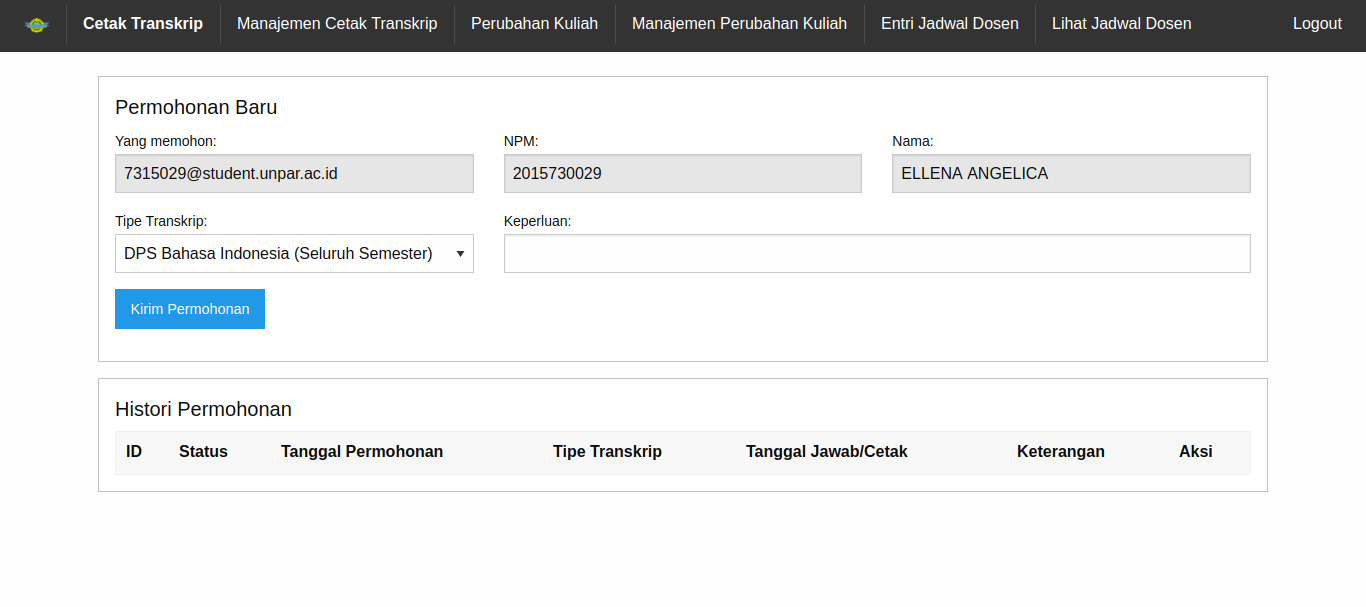
\includegraphics[width=\textwidth]{bluetape-cetak-transkrip.png}  
		\caption[Tampilan Cetak Transkrip]{Tampilan Cetak Transkrip} 
		\label{fig:bluetape-cetak-transkrip} 
	\end{figure}
	
	Gambar~ \ref{fig:bluetape-cetak-transkrip} menampilkan halaman utama saat cetak transkrip. Halaman ini hanya bisa diakses oleh \textit{user} yang termasuk roles 'root' dan 'mahasiswa.ftis'. Terdapat form yang meminta \textit{input} alamat \textit{email} pemohon, npm, nama, tipe transkrip, dan keperluan. Input alamat \textit{email} pemohon, npm, dan nama sudah terisi otomatis dan tidak bisa diubah lagi sehingga \textit{user} hanya perlu mengganti tipe transkrip dan mengisi keperluan. Tipe transkrip memiliki tiga pilihan, yaitu: DPS Bahasa Indonesia (Seluruh Semester), DPS Bahasa Inggris (Seluruh Semester), dan LHS (Semester Terakhir). Selain form tersebut, terdapat tabel histori permohonan yang akan menampilkan riwayat permohonan cetak transkrip jika sudah pernah memohon. Tabel histori permohonan memiliki tujuh kolom, yaitu: ID, Status, Tanggal Permohonan, Tipe Transkrip, Tanggal Jawab/Cetak, Keterangan, dan Aksi (tindakan yang bisa dilakukan dengan record). Gambar~ \ref{fig:bluetape-cetak-transkrip-request} menampilkan tampilan setelah form permohonan transkrip baru dikirimkan. Pada Gambar~ \ref{fig:bluetape-cetak-transkrip-request} aksi yang tersedia hanya melihat detail permohonan.

	\begin{figure}[H]
		\centering  
		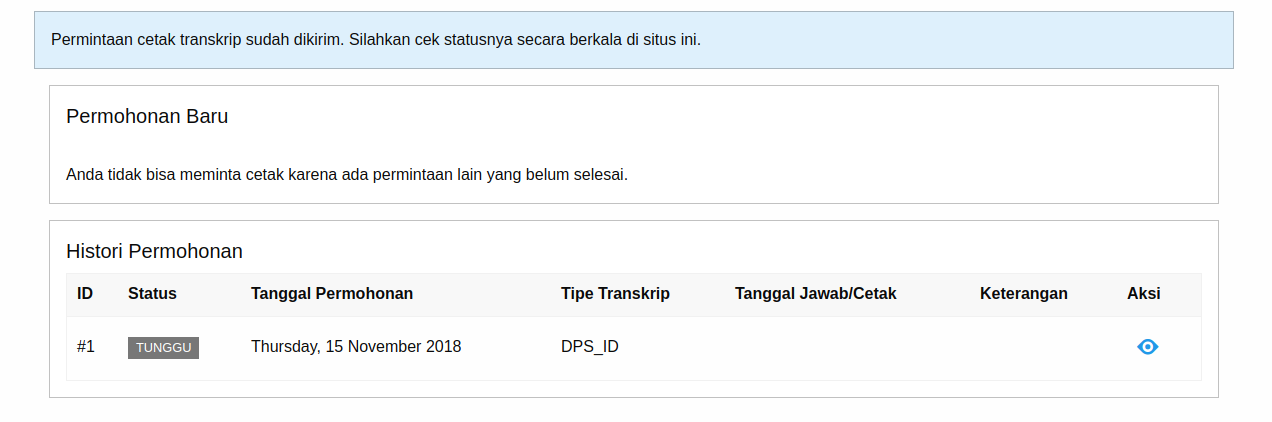
\includegraphics[width=\textwidth]{bluetape-cetak-transkrip-request.png}  
		\caption[Tampilan hasil Request Cetak Transkrip]{Tampilan hasil Request Cetak Transkrip} 
		\label{fig:bluetape-cetak-transkrip-request} 
	\end{figure}
	
	\subsubsection{Transkrip \textit{Manage}}
	\begin{figure}[H]
		\centering  
		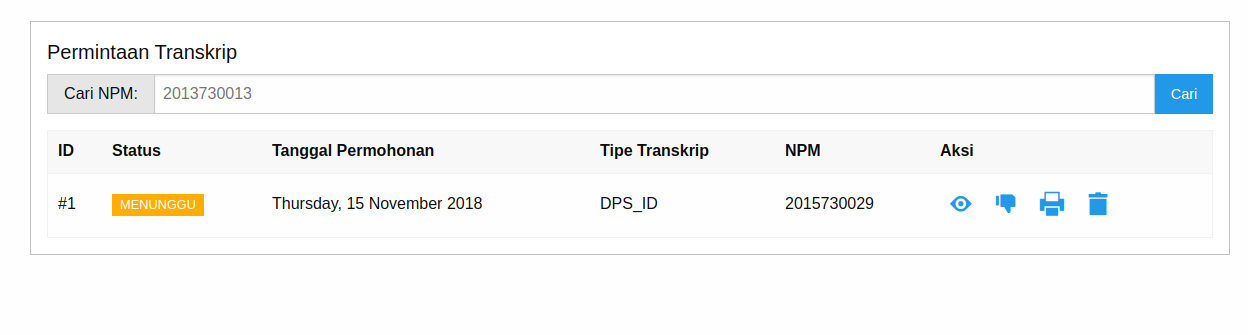
\includegraphics[width=\textwidth]{bluetape-manajemen-transkrip.png}  
		\caption[Tampilan Manajemen Transkrip BlueTape]{Tampilan Manajemen Transkrip BlueTape} 
		\label{fig:bluetape-manajemen-transkrip} 
	\end{figure}
	
	Gambar~ \ref{fig:bluetape-manajemen-transkrip} menampilkan tampilan halaman Manajemen Cetak Transkrip. Halaman ini hanya bisa diakses oleh \textit{user} yang termasuk roles 'root' dan 'tu.ftis'. Halaman ini memiliki kolom pencarian yang dapat diisi dengan npm mahasiswa. Angka "2013730013" pada Gambar~ \ref{fig:bluetape-manajemen-transkrip} merupakan placeholder saja, bukan \textit{input} \textit{user}. Apabila \textit{input} kosong, maka semua permohonan akan ditampilkan pada tabel di bawah kolom pencarian. Pada Gambar~ \ref{fig:bluetape-manajemen-transkrip}, permohonan yang masuk baru satu saja. Apabila \textit{input} diisi dan tombol "Cari ditekan", maka permohonan yang ditampilkan hanya permohonan milik npm yang diinput. User dapat melakukan empat aksi untuk tiap record yang ditampilkan: melihat detail permohonan (simbol mata), menolak permohonan (simbol jempol ke bawah), menyetujui permohonan (simbol \textit{print}), dan menghapus permohonan (simbol tempat sampah).
	
	\subsubsection{Perubahan Kuliah \textit{Request}}
	\begin{figure}[H]
		\centering  
		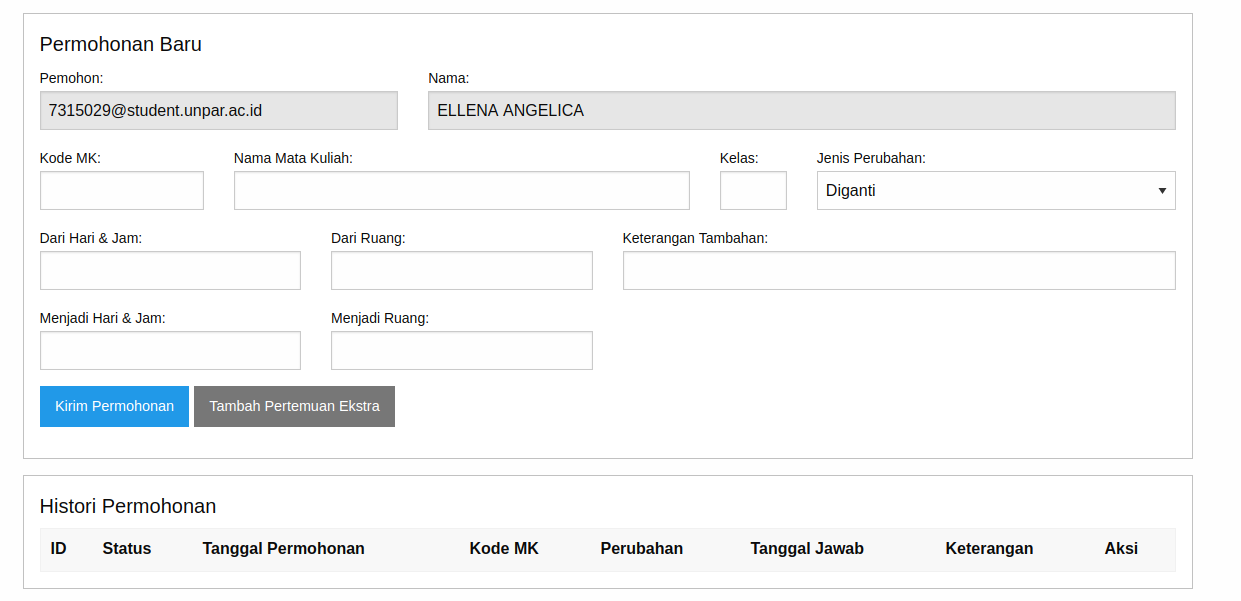
\includegraphics[width=\textwidth]{bluetape-perubahan-kuliah-request.png}  
		\caption[Tampilan request perubahan kuliah]{Tampilan request perubahan kuliah} 
		\label{fig:bluetape-perubahan-kuliah-request} 
	\end{figure}
	
	Gambar~ \ref{fig:bluetape-perubahan-kuliah-request} menampilkan halaman Perubahan Kuliah. Halaman ini hanya bisa diakses oleh \textit{user} yang termasuk roles 'root' dan 'staf.unpar'. Terdapat form yang meminta \textit{input} alamat \textit{email} pemohon, nama, kode mk, nama mata kuliah, kelas, jenis perubahan, hari dan jam sebelum dan sesudah diubah, serta ruang sebelum dan sesudah diubah. Input alamat \textit{email} pemohon dan nama sudah terisi otomatis dan tidak bisa diubah lagi. Jenis perubahan memiliki tiga pilihan, yaitu: diganti, tambahan, dan ditadakan. Selain form tersebut, terdapat tabel histori permohonan yang akan menampilkan riwayat permohonan perubahan jadwal kuliah. Tabel histori permohonan memiliki delapan kolom, yaitu: ID, Status, Tanggal Permohonan, Kode MK, Perubahan, Tanggal Jawab, Keterangan, dan Aksi (tindakan yang bisa dilakukan dengan record).
	
	\subsubsection{Perubahan Kuliah \textit{Manage}}
	\begin{figure}[H]
		\centering  
		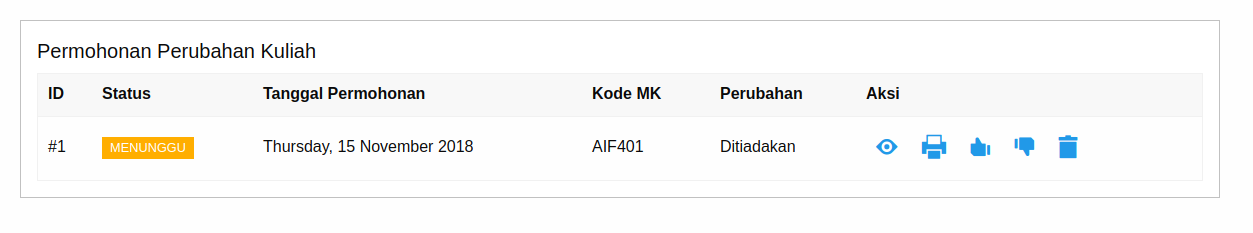
\includegraphics[width=\textwidth]{bluetape-perubahan-kuliah-manajemen.png}  
		\caption[Tampilan manage perubahan kuliah]{Tampilan manage perubahan kuliah} 
		\label{fig:bluetape-perubahan-kuliah-manajemen} 
	\end{figure}
	
	Gambar~ \ref{fig:bluetape-perubahan-kuliah-manajemen} menampilkan halaman Manajemen Perubahan Kuliah. Halaman ini hanya bisa diakses oleh \textit{user} yang termasuk roles 'root' dan 'tu.ftis'. Halaman ini berisi riwayat permohonan perubahan kuliah. User dapat melakukan empat aksi untuk tiap record yang ditampilkan: melihat detail permohonan (simbol mata), menolak permohonan (simbol jempol ke bawah), menyetujui permohonan (simbol print), dan menghapus permohonan (simbol tempat sampah).
	
	\subsubsection{Entri Jadwal Dosen}
	\begin{figure}[H]
		\centering  
		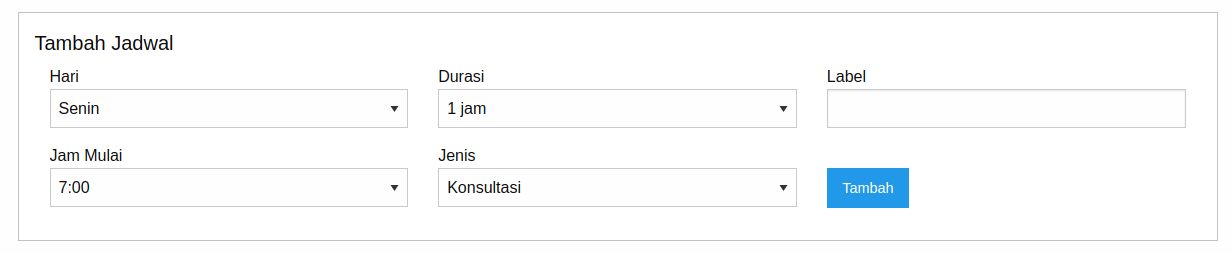
\includegraphics[width=\textwidth]{bluetape-entri-jadwal-dosen-tambah.png}  
		\caption[Tampilan tambah jadwal dosen]{Tampilan tambah jadwal dosen} 
		\label{fig:bluetape-entri-jadwal-dosen-tambah} 
	\end{figure}
	
	Gambar~ \ref{fig:bluetape-entri-jadwal-dosen-tambah}
	\begin{figure}[H]
		\centering  
		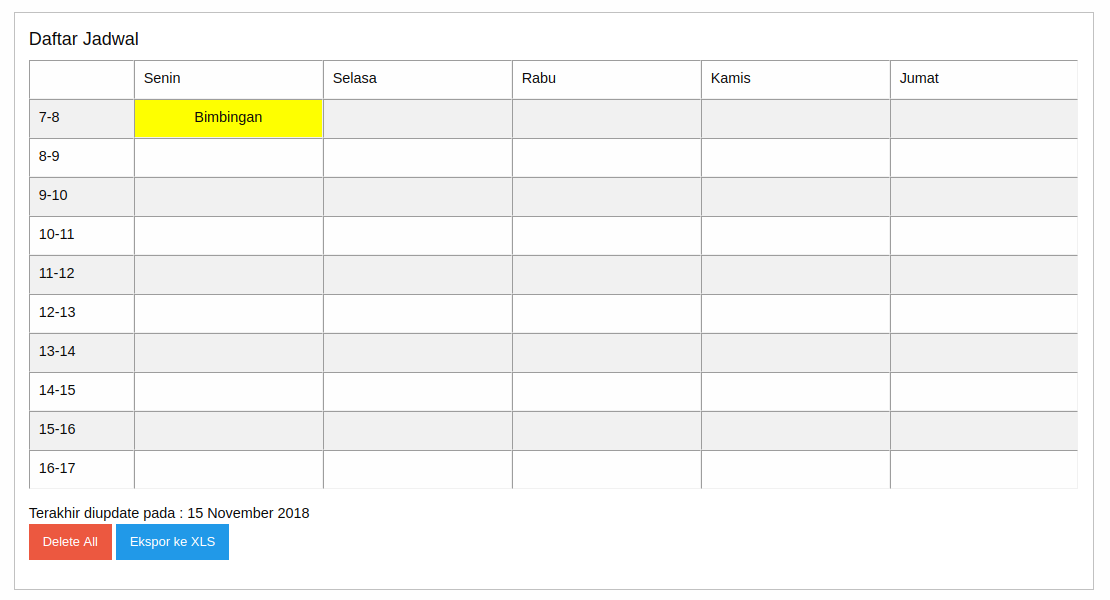
\includegraphics[width=\textwidth]{bluetape-entri-jadwal-dosen-daftar.png}  
		\caption[Tampilan jadwal dosen]{Tampilan jadwal dosen} 
		\label{fig:bluetape-entri-jadwal-dosen-daftar} 
	\end{figure}
	
	Halaman Entri Jadwal Dosen hanya bisa diakses oleh \textit{user} yang termasuk roles 'root' dan 'dosen.informatika'. Halaman ini terdiri dari dua bagian: form tambah jadwal dan daftar jadwal. Gambar~ \ref{fig:bluetape-entri-jadwal-dosen-tambah} menunjukkan form tambah jadwal. Form ini meminta \textit{input} hari, durasi, label, jam mulai dan jenis. Gambar~ \ref{fig:bluetape-entri-jadwal-dosen-daftar} menunjukkan daftar jadwal milik \textit{user}. Kolom yang memiliki isi bisa diklik untuk diedit. Gambar~ \ref{fig:bluetape-edit-jadwal-dosen} menunjukkan tampilan edit jadwal.
	
	\begin{figure}[H]
		\centering  
		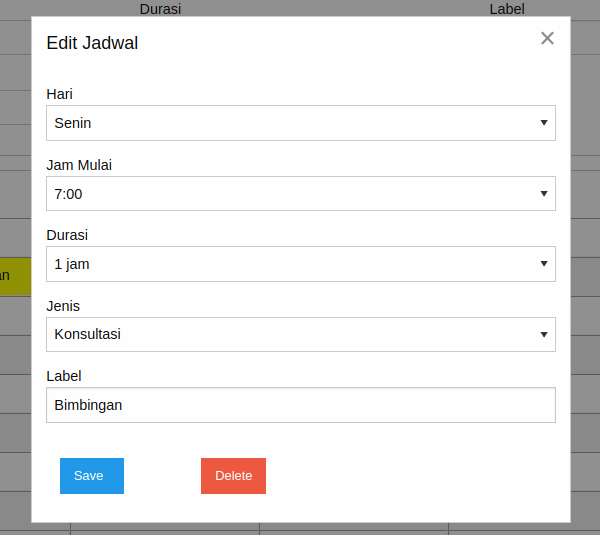
\includegraphics[scale=0.5]{bluetape-edit-jadwal-dosen.png}  
		\caption[Tampilan edit jadwal dosen]{Tampilan edit jadwal dosen} 
		\label{fig:bluetape-edit-jadwal-dosen} 
	\end{figure}

	\subsubsection{Lihat Jadwal Dosen}
	\begin{figure}[H]
		\centering  
		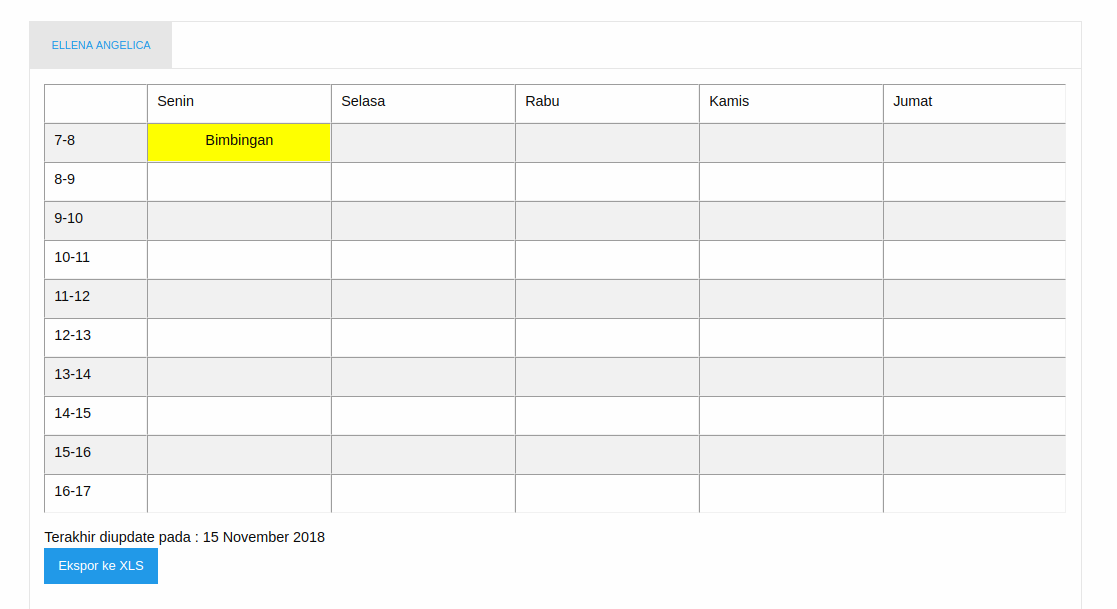
\includegraphics[width=\textwidth]{bluetape-lihat-jadwal-dosen.png}  
		\caption[Tampilan lihat jadwal dosen]{Tampilan lihat jadwal dosen} 
		\label{fig:bluetape-lihat-jadwal-dosen} 
	\end{figure}
	
	Gambar~ \ref{fig:bluetape-lihat-jadwal-dosen} menampilkan halaman Lihat Jadwal Dosen. Halaman ini bisa diakses oleh \textit{user} yang termasuk roles 'root', 'mahasiswa.informatika', dan 'dosen.informatika'. Halaman ini memiliki tab-tab yang masing-masing diberi label nama dosen. Di bawah tab terdapat tabel jadwal dari dosen yang tabnya aktif.

\subsection{Hak Akses}
	Hak akses dan nama \textit{module} diatur pada dokumen \texttt{config/modules.php} yang terletak di dalam direktori \texttt{config}. Hak akses dikelompokkan di dalam kelompok yang disebut \textit{role}. Saat skripsi ini dibuat, hak akses dibagi ke dalam lima \textit{role}: root, mahasiswa.ftis, tu.ftis, staf.unpar, dosen.informatika, dan mahasiswa.informatika. \textit{Role} root berisi daftar alamat \textit{email} dari pengembang bluetape. \textit{Role} tu.ftis berisi daftar alamat \textit{email} dari tata usaha ftis. \textit{Role} mahasiswa.ftis berisi daftar alamat \textit{email} dari mahasiswa ftis. \textit{Role} staf.unpar berisi daftar alamat \textit{email} dari staf unpar. \textit{Role} dosen.informatika berisi daftar alamat \textit{email} dari dosen informatika.

	Setiap \textit{role} memiliki batasan dalam mengakses \textit{module} di BlueTape. \textit{Role} root tidak memiliki batasan dan dapat mengakses setiap \textit{module} yang ada. \textit{Role} tu.ftis hanya dapat mengakses \textit{module} \texttt{TranskripManage}, dan \textit{module} \texttt{PerubahanKuliahManage}. \textit{Role} mahasiswa.ftis hanya dapat mengakses \textit{module} \texttt{TranskripRequest} dan \textit{module} \texttt{LihatJadwalDosen}. \textit{Role} staf.unpar hanya dapat mengakses \textit{module} \texttt{PerubahanKuliahRequest}. \texttt{Role} dosen.informatika hanya dapat mengakses \textit{module} \texttt{EntriJadwalDosen}.

\section{Analisis Fitur yang Dibangun}
\label{sec:analisisYangDibangun}
	Bagian ini membahas analisis fitur kolektor pengumuman.

\subsection{Diagram \textit{Use Case}}
\begin{figure}[H]
	\centering  
	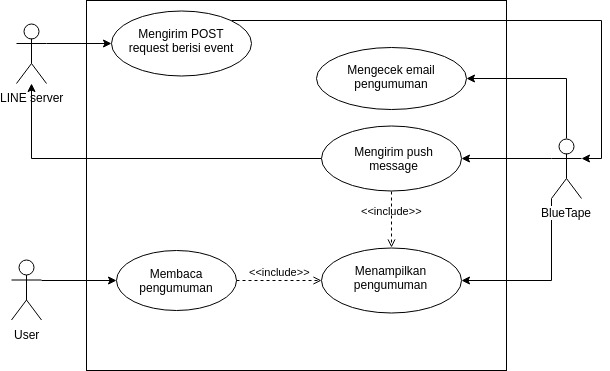
\includegraphics[width=\textwidth]{use-case-diagram.jpg}  
	\caption[Use case diagram fitur kolektor pengumuman]{Use case diagram fitur kolektor pengumuman} 
	\label{fig:use-case-diagram} 
\end{figure}

Gambar~\ref{fig:use-case-diagram} merupakan gambar diagram \textit{use case} fitur kolektor pengumuman. Pada diagram \textit{use case} fitur kolektor pengumuman terdapat tiga aktor: dosen informatika, mahasiswa informatika, dan root (admin). Berikut ini adalah penjelasan dari skenario pada diagram \textit{use case} tersebut:
\begin{enumerate}
\item Menerbitkan pengumuman via \textit{email}

\begin{itemize}
	\item Aktor: Dosen Informatika.
	\item Skenario Normal

	\begin{enumerate}
		\item Dosen mengirimkan \textit{email} ke alamat \textit{email} yang dikhususkan untuk menampung pengumuman di jurusan Teknik Informatika.
		\item BlueTape mengecek \textit{email} tersebut pada periode tertentu.
		\item Jika alamat \textit{email} yang dosen pakai terdaftar di BlueTape, maka BlueTape akan menampilkannya dan mengirim notifikasi ke LINE.
	\end{enumerate}
	
	\item Skenario Exception
	\begin{enumerate}
		\item Dosen mengirimkan \textit{email} ke alamat \textit{email} yang dikhususkan untuk menampung pengumuman di jurusan Teknik Informatika.
		\item BlueTape mengecek \textit{email} tersebut pada periode tertentu.
		\item Jika alamat \textit{email} yang dosen pakai tidak terdaftar di BlueTape, maka BlueTape akan mengabaikan \textit{email} tersebut.
	\end{enumerate}
\end{itemize}

\item Mendaftar sebagai penerima notifikasi pengumuman di LINE

\begin{itemize}
	\item Aktor: Mahasiswa Informatika.
	\item Skenario Normal

	\begin{enumerate}
		\item Mahasiswa mengikuti bot BlueTape dengan menambahkannya sebagai teman.
		\item Bot BlueTape akan mengirim notifikasi kepada mahasiswa jika ada pengumuman baru di BlueTape.
	\end{enumerate}
\end{itemize}

\item Menerima notifikasi pengumuman di LINE

\begin{itemize}
	\item Aktor: Mahasiswa Informatika.
	\item Skenario Normal

	\begin{enumerate}
		\item Mahasiswa menerima notifikasi dari bot BlueTape saat ada pengumuman baru di BlueTape.
		\item Mahasiswa mengunjungi URL yang dicantumkan di pesan dari notifikasi tersebut. 
		\item Mahasiswa perlu \textit{login} menggunakan \textit{email} \textit{student} miliknya terlebih dahulu sebelum dapat mengunjungi URL tersebut.
	\end{enumerate}
\end{itemize}

\item Melihat pengumuman terkirim di dashboard

\begin{itemize}
	\item Aktor: Dosen Informatika, Mahasiswa Informatika, dan root (admin).
	\item Skenario Normal

	\begin{enumerate}
		\item Dosen Informatika, Mahasiswa Informatika, atau root (admin) mengunjungi menu Pengumuman. Menu Pengumuman berisi daftar pengumuman yang masuk ke BlueTape. Daftar tersebut disortir dari yang paling baru.
		\item Saat salah satu pengumuman diklik, maka isi dan detail pengumuman tersebut akan ditampilkan.
	\end{enumerate}
\end{itemize}
\end{enumerate}

\subsection{Arsitektur Heroku yang digunakan untuk Bluetape}
	\subsubsection{\textit{Dependency}}
		BlueTape membutuhkan \textit{dependency} tambahan agar perangkat lunak dapat dijalankan. \textit{Dependency} tambahan perangkat lunak BlueTape tertera pada dokumen \texttt{composer.json}. Berikut isinya:
		\begin{lstlisting}
		{
		    "require": {
		        "google/apiclient": "^1.0",
				"ext-imap": "*",
		        "phpoffice/phpexcel": "^1.8",
		        "linecorp/line-bot-sdk": "^3.6"
		    }
		}
		\end{lstlisting}
		
		Pada saat skripsi ini ditulis, BlueTape telah memakai dua \textit{package}: \textit{package} \texttt{google/apiclient} dan \textit{package} \texttt{phpoffice/phpexcel}. \textit{Package} \texttt{google/apiclient} adalah \textit{package} yang diperlukan untuk autentikasi akun saat masuk ke BlueTape. Sedangkan \textit{package} \texttt{phpoffice/phpexcel} adalah \textit{package} yang digunakan untuk menghasilkan dokumen excel. \textit{Package} yang diperlukan untuk skripsi ini adalah \textit{package} \texttt{ext-imap} dan \texttt{line-bot-sdk}. \textit{Package} \texttt{ext-imap} digunakan untuk mengakses \textit{email}. \textit{Package} \texttt{line-bot-sdk} digunakan untuk menghubungkan perangkat lunak dengan layanan yang disediakan oleh LINE.
		
	\subsubsection{\textit{Process Type}}
		BlueTape hanya membutuhkan satu \textit{process type} di Procfile, yaitu \textit{process type} \texttt{web} dan \textit{process type} \texttt{release}. \textit{Process type} \texttt{web} adalah \textit{process type} yang digunakan untuk menerima arus HTTP eksternal dari router Heroku.
		
	\subsubsection{Procfile}
		Procfile adalah \textit{file} yang menjelaskan Heroku bagian-bagian perangkat lunak yang dapat dieksekusi. Procfile berisi daftar \textit{process type} beserta cara menjalankannya. BlueTape hanya memiliki satu \textit{process type}, yaitu \textit{process type} \texttt{web}. Isi Procfile adalah:
		\begin{lstlisting}
		web: vendor/bin/heroku-php-apache2 www/
		\end{lstlisting}
		
		Maksud dari satu baris Procfile tersebut adalah: untuk menjalankan \textit{process type} web, heroku harus menjalankan \textit{server apache} di Heroku dan kemudian \textit{server} menjalankan aplikasi web yang ada di direktori \texttt{www}. Perintah \texttt{vendor/bin/heroku-php-apache2} adalah perintah untuk menjalankan \textit{server apache} di heroku yang ada di \textit{package} \texttt{heroku-php-apache2}. \textit{Package} \texttt{heroku-php-apache2} ini otomatis disediakan saat membuat perangkat lunak php di heroku sehingga tidak perlu ditambahkan di composer.json. Perintah \texttt{www/} berguna untuk mengarahkan \textit{server apache} heroku ke direktori \texttt{www}.
		
	\subsubsection{\textit{Slug}}
		Pada skripsi ini, \textit{file} \texttt{.slugignore} tidak perlu ditambahkan karena tidak diperlukan.
		
	\subsubsection{\textit{Buildpack}}
	\textit{Buildpack} yang dipakai pada skripsi ini cukup hanya \texttt{heroku/php}. \textit{Buildpack} ini secara otomatis akan dipakai oleh Heroku karena BlueTape memakai bahasa PHP.
		
	\subsubsection{\textit{Dyno}}
		Jenis \textit{dyno} yang dipakai pada skripsi ini adalah \textit{free dyno}. Jumlah \textit{dyno} hanya satu. \textit{Dyno} tersebut merupakan \textit{dyno} untuk \textit{process type} \texttt{web}.
		
	\subsubsection{\textit{Config Vars}}
		\textit{Environment variable} yang perlu disimpan di \textit{config vars} adalah konfigurasi \textit{basis data}, konfigurasi autentikasi dengan OAuth Google, konfigurasi autentikasi \textit{email} kolektor pengumuman, konfigurasi aplikasi, dan konfigurasi untuk terhubung ke LINE.
		
		Berikut adalah nama-nama \textit{config vars} yang akan dipakai pada skripsi ini beserta keterangannya: 
		\begin{itemize}
			\item CI\_DB\_DATABASE: nama \textit{database} yang digunakan.
			\item CI\_DB\_HOSTNAME: nama \textit{host} dari \textit{database} yang disebutkan di \textit{config var} CI\_DB\_DATABASE.
			\item CI\_DB\_USERNAME: \textit{username} yang digunakan untuk terhubung ke \textit{database} yang disebutkan di \textit{config var} CI\_DB\_DATABASE.
			\item CI\_DB\_PASSWORD: \textit{password} dari \textit{username} yang disebutkan di \textit{config var} CI\_DB\_USERNAME.
			\item HEROKU\_POSTGRESQL\_BLUE\_URL: URL \textit{database}. Dibuat secara otomatis saat membuat \textit{database}.
			\item GOOGLE\_CLIENTID: Google Client ID, digunakan untuk melakukan autentikasi saat \textit{user} \textit{login}.
			\item GOOGLE\_CLIENTSECRET: Google Client Secret, digunakan untuk melakukan autentikasi saat \textit{user} \textit{login}.
			\item ANNOUNCEMENT\_EMAIL: alamat \textit{email} yang dipakai untuk menampung pengumuman.
			\item ANNOUNCEMENT\_PASSWORD: \textit{password} untuk alamat \textit{email} yang disebutkan di \textit{config var} ANNOUNCEMENT\_EMAIL.
			\item HOSTNAME\_INCOMING\_EMAIL: nama \textit{host} dari alamat \textit{email} yang disebutkan di \textit{config var} ANNOUNCEMENT\_EMAIL.
			\item CI\_BASE\_URL: \textit{base} URL BlueTape.
			\item LINE\_BOT\_CHANNEL\_SECRET: LINE Bot Channel Secret digunakan untuk terhubung ke \textit{channel bot} untuk pengumuman.
			\item LINE\_BOT\_CHANNEL\_TOKEN: LINE Bot Channel Token digunakan untuk terhubung ke \textit{channel bot} untuk pengumuman.
			\item SMTP\_HOST: SMTP \textit{host}, konfigurasi untuk mengirim \textit{email}.
			\item SMTP\_PASS: SMTP \textit{pass}, konfigurasi untuk mengirim \textit{email}.
			\item SMTP\_PORT: SMTP \textit{port}, konfigurasi untuk mengirim \textit{email}.
			\item SMTP\_USER: SMTP \textit{user}, konfigurasi untuk mengirim \textit{email}.
		\end{itemize}
		
	\subsubsection{\textit{Region}}
	\textit{Region} yang dipakai adalah \textit{region default}, yaitu \textit{United States}.
		
	\subsubsection{\textit{Stack}}
	\textit{Stack} yang dipakai adalah \textit{stack} yang paling baru, yaitu heroku-18. \textit{Stack} ini dipilih karena Heroku masa kadaluarsa dukungan untuk \textit{stack} ini yang paling lama (didukung sampai bulan April 2023). Alasan lain adalah komputer lokal yang digunakan untuk mengerjakan skripsi ini menggunakan lingkungan yang mirip dengan Heroku, yaitu menggunakan Ubuntu 18.04.

	\subsubsection{Basis Data}
		Basis data yang digunakan untuk skripsi ini adalah basis data Heroku Postgres dengan plan \textit{hobby-dev}. Alasan basis data ini digunakan adalah karena basis data ini adalah basis data yang secara otomatis disediakan oleh Heroku dan fiturnya cukup untuk digunakan oleh BlueTape.
	
		Sebelumnya BlueTape menggunakan MySQL untuk basis datanya. Proses migrasi dari MySQL ke Heroku Postgres tidak rumit, karena menggunakan fitur \textit{Migration} dari CodeIgniter. Namun, ada beberapa perubahan pada dokumen \textit{Migration}. Perubahan-perubahan tersebut adalah:
	\begin{itemize}
		\item Menyelaraskan nama tabel karena sifat case sensitive pada Postgres
		\item Mengubah Replace menjadi Insert dan Update karena Replace tidak didukung oleh Postgres
		\item Mengubah tipe data kolom yang sebelumnya menggunakan DATETIME menjadi timestamp
	\end{itemize}  

\subsection{Sinkronisasi \textit{Email}}
\label{sec:analisisemail}
	Awalnya sinkronisasi \textit{email} akan dilakukan dengan memanfaatkan Gmail API. Namun, Gmail API membutuhkan \textit{token} yang harus diperbarui tiap periode tertentu. Jika peneliti ingin \textit{token} dapat diperbarui, maka \textit{file refresh token} harus disimpan di Heroku. Namun, Heroku memiliki \textit{filesystem} yang tidak mendukung penyimpanan \textit{file} yang berubah-ubah. Sehingga, peneliti perlu mencari alternatif lain. Peneliti memutuskan menggunakan PHP IMAP untuk melakukan sinkronisasi \textit{email}.
	
	Sebelum melakukan sinkronisasi \textit{email}, \textit{email} khusus untuk menampung \textit{email} pengumuman harus dibuat terlebih dahulu. \textit{Email} dibuat melalui \textit{provider} \textit{email} Gmail. Setelah \textit{email} selesai dibuat, fitur IMAP perlu dinyalakan terlebih dahulu.
	
	Proses sinkronisasi \textit{email} dimulai dengan membuat koneksi IMAP ke \textit{email} pengumuman tersebut. Dengan menggunakan koneksi IMAP yang telah didapat, \textit{email} difilter dengan mencari \textit{email} yang belum dibaca saja. Apabila hasil pencarian tidak kosong, maka setiap \textit{email} pada hasil pencarian akan diperiksa pengirimnya. Pengirim \textit{email} akan dinyatakan sebagai pemberi pengumuman yang sah apabila ia terdaftar di dalam daftar pengirim yang terverifikasi. Apabila sebuah \textit{email} dinyatakan memiliki pengirim yang sah, maka informasi dari \textit{email} tersebut akan diproses dan dimasukkan ke basis data.
	
	Informasi yang perlu disimpan dari \textit{email} pengumuman adalah alamat \textit{email} pengirim, nama pengirim, tanggal \textit{email} tersebut terkirim, subjek \textit{email}, isi \textit{email}, dan ketersediaan lampiran. Sebuah tabel baru diperlukan untuk menampung informasi ini. Tabel ini akan diakses saat halaman pengumuman akan ditampilkan. Setiap informasi dari \textit{email} tersimpan, maka satu \textit{push message} akan dikirim ke LINE.
	
	Sinkronisasi \textit{email} perlu dilakukan secara berkala dan otomatis. Pada skripsi ini sinkronisasi \textit{email} dilakukan per hari dengan menggunakan \textit{cron} dan \textit{add-on} Heroku Scheduler.
	
\subsection{Menghubungkan BlueTape dengan LINE}
\label{sec:analisisline}
	Produk LINE yang digunakan untuk menghubungkan BlueTape dengan LINE adalah LINE Messaging API. Produk ini paling memenuhi kriteria fitur kolektor pengumuman, yaitu dapat mengirimkan \textit{push message}.
	
	Sebelum menghubungkan BlueTape dengan LINE, ada beberapa hal yang harus dilakukan terlebih dahulu di LINE Developers \textit{console}. Pertama, membuat akun LINE dan mendaftar sebagai developer di LINE Developers \textit{console}. Kedua, membuat \textit{provider} di LINE Developers \textit{console}. Ketiga, membuat \textit{channel} pada \textit{provider} tersebut. \textit{Channel} yang dibuat harus menggunakan \textit{plan Developer Trial} karena \textit{plan} ini yang memiliki fitur \textit{push message}. Setelah \textit{channel} terbuat, sebuah akun \textit{bot} otomatis dibuat.
	
	Pada \textit{channel}, terdapat tiga bagian penting: \textit{channel access token, channel secret}, dan \textit{webhook URL}. \textit{Channel access token} dan \textit{channel secret} digunakan untuk autentikasi saat aplikasi BlueTape dan LINE berinteraksi. Kedua kode ini dapat diubah-ubah menggunakan tombol \textit{issue} pada masing-masing kolom. Sedangkan \textit{webhook URL} adalah alamat URL untuk menerima POST \textit{request} berisi \textit{event-event} yang terjadi pada \textit{bot}. Contoh: \textit{event following} yang terjadi saat ada akun LINE yang \textit{follow} atau menambah akun bot sebagai teman. \textit{Webhook URL} dapat diubah-ubah, namun harus menggunakan alamat https. Selain itu, fitur \textit{csrf protection} milik Codeigniter harus dimatikan pada alamat URL tersebut.
	
	Pada skripsi ini, tidak semua \textit{event} perlu ditangani. Event yang harus ditangani cukup \textit{follow event} dan \textit{unfollow event}. Saat \textit{follow event} terjadi, \textit{user id} dari akun \textit{follower} akan disimpan di sebuah tabel di basis data. Apabila \textit{user id} memblokir akun bot sehingga \textit{unfollow event} terjadi, maka \textit{user id} tersebut dihapus dari tabel. Penyimpanan ini diperlukan karena \textit{user id} diperlukan saat mengirim \textit{push message} dan tidak ada fungsi pada line-bot-sdk untuk mendapatkan \textit{user id follower} akun \textit{bot}.